\documentclass[../main.tex]{subfiles}
\graphicspath{{\subfix{../imgs/}}}
\begin{document}
\thispagestyle{plain}
\newpage

\section{The Model}

\subsection{Background}

In the landmark paper "Attention Is All You Need" \cite{Vaswani:1}, Vaswani et al. propose the Transformer model as an alternative to previous state-of-the-art sequence transduction models. These include Recurrent Neural Networks (RNNs), Long Short-Term Memory (LSTMs) \cite{Hochreiter:1} and Gated RNNs \cite{Chung:1} built with encoder-decoder architectures for sequence-to-sequence generation. Recurrent models typically handle computation based on the positions of symbols in input and output sequences. By aligning these positions with computational time steps, they generate a series of hidden states where the most recent hidden state, $ht$, depends on the previous hidden state, $ht-1$, and the input for the current position (t).

This sequential nature inherently restricts parallelization and is especially true for longer sequences where memory limitations constrain the ability to batch multiple examples together. Recent research has made notable strides in improving computational efficiency through methods like factorization techniques \cite{Kuchaiev:1} and conditional computation \cite{Shazeer:1} while also enhancing model performance, particularly in the case of the latter approach. Many of these models also employ attention mechanisms, which allow some amount of modeling of input sequence dependencies without regard to their distance in the input/output sequence \cite{Kim:1}. Nonetheless, the core constraint of sequential computation imposed by recurrent neural networks has remained.  

The transformer model, however, does away with recurrence entirely and relies solely on attention mechanisms to draw global relationships between input and output. This makes the Transformer model highly parallelizable for faster, more efficient training.

\subsection{Model Structure}
Similar to prior state-of-the-art sequence transduction models, the transformer has an encoder-decoder structure where the encoder maps an input sequence of representations $X = (x_1, ... x_n)$ to some sequence of continuous feature representations $Z = (z_1, ... z_n)$. Provided with these continuous feature representations $Z$, the decoder can generate an output sequence one element at a time, using previously generated symbols as additional input to generate subsequent symbols. The Transformer uses a similar overall architecture but instead uses stacked self-attention layers and fully connected layers in both the encoder and decoder, as shown in Figure \ref{fig:fig1}.

\begin{figure}[hp]
    \centering
    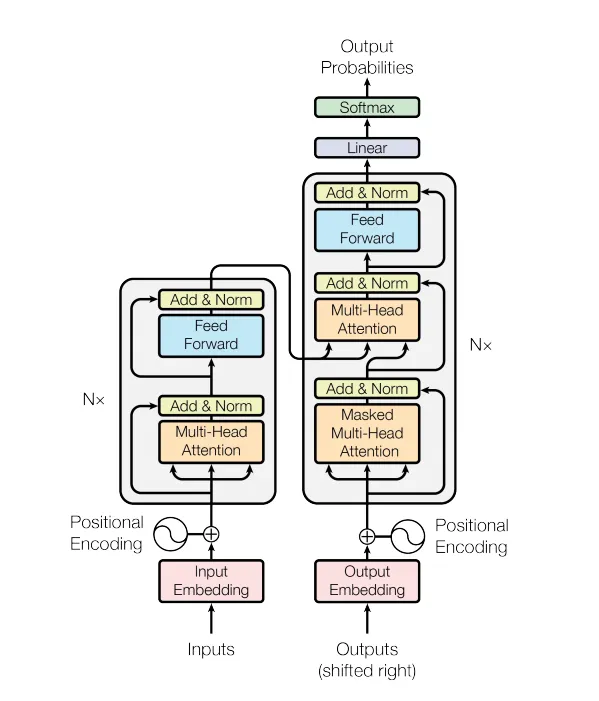
\includegraphics[width=1\textwidth]{imgs/transformer.png}
    \caption{The Transformer Model Architecture (Taken directly from Vaswani et al.)}
    \label{fig:fig1}
\end{figure}

\subsection{Inputs and Embeddings}
The input to a Transformer consists of a sequence of tokens. The tokens can be words, characters, numbers, or any other kind of symbol that inherently holds sequential logic. Before being fed into the model, these tokens are embedded into continuous vector representations — \textit{feature vectors} — using an embedding layer such that each token is now represented by a unique vector. These input embeddings can be learned by the model during training. More commonly, we reuse learned input embeddings created by other models that may be trained on much larger data sets. 

\subsection{Positional Encoding}
Unlike Recurrent Neural Networks, the self-attention mechanism of the Transformer creates a new problem: our input sequence no longer inherently holds positional information. To encode position into our input, Vaswani et al. propose a means to "inject" positional information about the tokens in our sequence. This is done by adding "positional encodings" to the input embeddings directly. Vaswani et al. use sinusoidal functions of different frequencies to encode position into each token's embedding:

{\large
\begin{align*} 
\label{eq:1.1}
PE_{(pos,2i)} = sin(pos/10000^{2i/d_{model}} ) \\
PE_{(pos,2i+1)} = cos(pos/10000^{2i/d_{model}} )
\tag{1.1}
\end{align*}
}

where \textit{pos} is the position in the token and \textit{i} is the dimension of the positional encoding that corresponds to a sinusoidal function. 


\subsection{Encoder / Decoder Stacks }

\textbf{Encoder} — The encoder is composed of a stack of 6 identical layers, each with 2 sub-layers. The first is a multi-head self-attention layer, followed by a fully connected feed-forward network. Each sub-layer has a residual connection, followed by layer normalization where the output of each sub-layer is $Normalize(x + sublayer(x))$. To facilitate this, all sub-layers in the model as well as the embedding layers output tensors of dimensions $d_{model}$, which is 512 for their implementation.

\vspace{0.5cm} \noindent
\textbf{Decoder} — The decoder is also composed of a stack of 6 identical layers. In addition to the two sub-layers in each encoder layer, the decoder inserts a second multi-head attention in the middle which acts on the output of the encoder stack. The multi-head attention sub-layer in the decoder stack is also modified to prevent positions from attending to subsequent positions with an input mask. This combined with the fact that the output embeddings are offset by one position, ensures that the predictions for any position $pos_i$ can depend only on positions $pos_k$ where $k<i$. Like the Encoder stack, we similarly employ residual connections and layer normalization around each sub-layer

\subsection{Attention}

\subsubsection{Self-Attention}
The self-attention function is at the core of the transformer and is the reason for the transformer's huge success in the field of NLP. The self-attention mechanism is what allows the model to be heavily parallelized, and also allows the model to draw relationships between tokens across the entire length of the input sequence in constant time. The auto-regressive nature of self-attention makes this mechanism particularly great for music, which is often composed of recurring structures that repeat and develop. 

Similar to many modern-day search engines, an attention function can be described as mapping a query and a set of key-value pairs to some output, where each of these — the query, keys, values, and output — are vectors. The output is computed as the weighted sum of each matched value, where the weight assigned to each value is dependent on a "similarity" function that compares the query against the corresponding key. 

\begin{itemize}
    \item \textbf{Queries, Keys, and Values:} Each input token is associated with three vectors: \textit{Query (Q), Key (K), and Value (V)}. These vectors are learned during training.

    \item \textbf{Attention Scores:} For each token in the sequence, the self-attention mechanism calculates an attention score by measuring the similarity between its Query vector and the Key vectors of all other tokens.

    \item \textbf{Weighted Sum:} The attention scores determine how much of every other token in the sequence contributes to the output for the current token. This is achieved with a weighted sum of each token's Value vectors, producing the context vector as output for the current token.
\end{itemize}


\subsubsection{Multi-Head Attention}
Instead of performing a single attention function over the entire Query, Key, and Value vectors of dimension $d_{model}$, Vaswani et al. propose a linear projection of the queries, keys, and values $h$ times to $d_{query}$, $d_{key}$, $d_{value}$ dimensions respectively. This is achieved by placing linear layers before the multi-head attention layer and projecting the queries, keys, and values in a smaller space. On each of these projected versions of queries, keys, and values we then perform the attention function in parallel, yielding $d_v$ dimension output values. This allows us to capture multiple relationships between tokens as the model can attend to information between different representation subspaces at different positions. The output of each of these 'heads' is a vector of dimension $d_k$, which are concatenated and once again projected to get our final output. 

{
    \begin{align*}
    \label{eq:1.2}
    MultiHead (Q,K,V) = Concat(head_1, .... head_h)W^O \\
    head_i = Attention(QW^Q_i, KW^K_i, VW^V_i) 
    \tag{1.2}
    \end{align*}
}

where the projections are done via the following parameter matrices:

{
\large
\begin{align*}
W^Q_i \in R^{\ {d_{model} \ \times \ d_k}} \\
W^K_i \in R^{\ {d_{model} \ \times \ d_k}} \\
W^V_i \in R^{\ {d_{model} \ \times \ d_v}} \\
W^O \in R^{\ {hd_v \ \times \ d_{model}}}
\end{align*}
}

\subsubsection{Scaled Dot-Product Attention}

\begin{figure}[htpb]
    \centering
    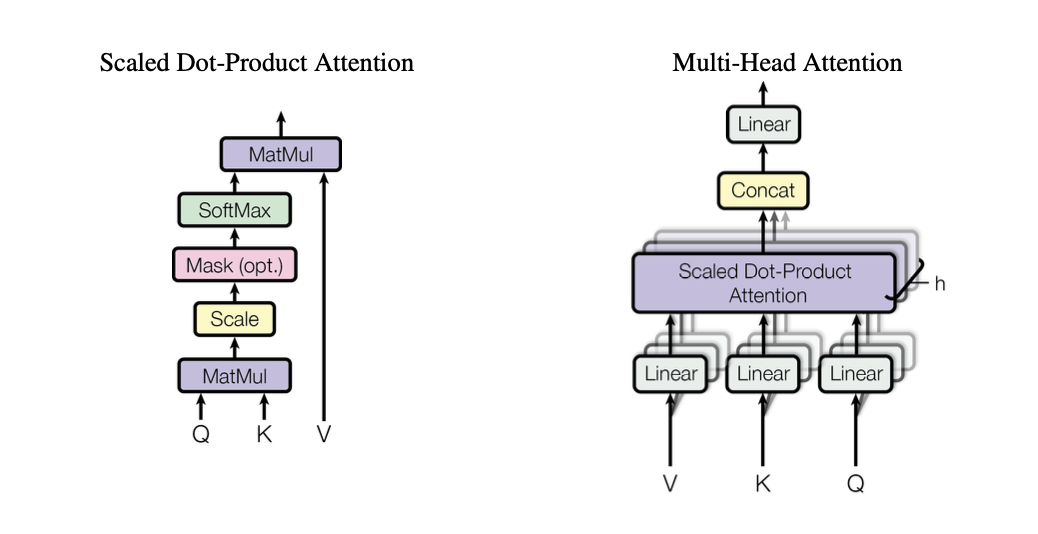
\includegraphics[width=1\textwidth]{imgs/scaled_dot_product_attention.png}
    \caption{(left) Scaled Dot-product Attention. (Right) Multi-head Attention with several layers in parallel. Taken directly from Vaswani et al.}
    \label{fig:fig2}
\end{figure}

In particular, the form of attention implemented by Vaswani et al. is Scaled-Dot-Product Attention\ref{fig:fig2} First the dot products of the query with all the keys are calculated. It is then divided by $\sqrt{d_k}$ — to counter dot-product values growing too large, resulting in vanishing gradients — and converted to a probability distribution by applying a softmax function to obtain weights on the values. As described earlier, the attention function is computed on a set of multiple queries, keys, and values simultaneously, packed in matrices Q, K, and V respectively.

{\large
\[
\label{eq:1.3}
Attention (Q,K,V) = softmax(\frac {QK^T} {\sqrt{d_k}})V 
\tag{1.3}
\]}

\subsection{Position-Wise Feed Forward Networks}
In addition to attention sub-layers, each of the layers in our encoder and decoder contains a fully connected feed-forward network, which is applied to each position separately and identically. This consists of two linear transformations with a ReLU activation in between:

\[ FFN(x) = max(0, xW_1 + b_1 )W_2 + b_2 (2) \]

where $W_1, W_2$ and $b_1, b_2$ are weights and biases of each linear layer respectively. In the case of Vaswani et al., the dimensionality of input and output is $d_{model}$ = 512, and the inner layer has dimensionality $d_{ff}$ = 2048.

\newpage
\section{Proposed Modifications to the Baseline Transformer Model}

\subsection{Considerations}
Given the fact that we are applying the Transformer model to an entirely different domain of music, we must consider the differences between the domains of music and language to make modifications to our transformer model accordingly. One key issue is in the matter of positional encoding. In its original state, the Transformer model above relies on absolute position representations using positional sinusoids that are added to the input embeddings at each input position. This is very different from state-of-the-art models, usually RNNs and LSTMs, which instead model positions in relative terms. %CITATION NEEDED HERE.
Furthermore, working with music dramatically alters the input our model might receive. 

\newpage
\subsection{Relative Positional Self-Attention}
Music has two dimensions along which relative differences matter more than absolute differences: Time and Pitch. This key information is captured in the event-based input representation proposed by Oore et al. 

To capture such pairwise relationships between representations, Shaw et al. \cite{shaw:1} introduce a version of the self-attention mechanism that is regulated by the distance between two points, which involves learning a separate relative position embedding $E^r$ of shape $(h,l,d_k)$, where $h$ is the number of heads, $l$ is the length of the input sequence, and $d_k$ is the dimensionality of the projected keys, queries and values that are fed to each head in the multi-head attention layer. $E^r$ holds an embedding of each possible pair-wise distance $r = i_q - j_k$ between a query and key in position $i_q$ and $j_k$ respectively. 

These are ordered from $-L + 1$ to $0$ and are learned separately for each head. As proposed in Shaw et al, the relative embeddings interact with queries to give rise to $S^{rel}$, and $L \times L$ dimensional logits matrix that can be used to modulate attention probabilities for each head. 

{
\begin{align*}
\label{eq:1.4}
Absolute Attention (Q,K,V) = softmax(\frac {QK^T} {\sqrt{d_k}})V \\ \\
Relative Attention (Q,K,V) = softmax(\frac {QK^T + S^{rel}} {\sqrt{d_k}})V
\tag{1.4}
\end{align*}
}

For each head, Shaw et al. create a temporary tensor $R$ of shape $(L, L, d_k)$, containing the embeddings that correspond to the relative distances between all keys and queries. Q is then reshaped to an $(L, 1, d_k)$ tensor, and $S^{rel} = QR^T$ This incurs a total space complexity of $O(L^2D)$, restricting its application to long sequences, and making the model less feasible for real-time generation tasks. 

However, Huang et al. \cite{Huang:1} propose a memory-efficient implementation of relative attention by reducing the intermediate memory requirement to $O(LD)$. Huang et al. observe that all of the terms we need from $QR^{T}$ are already available when $Q$ is directly multiplied with $E^r$, the relative positional embedding. After we compute $Q{E^{r}}^{T}$, its $(i_q,r)$ entry contains the dot product of the query in position $i_q$ with the embedding of relative distance $r$. Each relative logit $(i_q, j_k)$ in the matrix $S^{rel}$ from Equation \ref{eq:1.4} should be the dot product of the query in position $i_q$ and the embedding of the relative distance $i_q-j_k$, to match up with the indexing in $Q^{K^{T}}$. 

We therefore need to “skew” $Q{E^{r}}^{T}$ to move the relative logits to their correct positions. The “skewing” procedure is illustrated in Figure \ref{fig:fig4} below and is detailed in Huang et al. \cite{Huang:1} The time complexity for both methods is $O(L^2D)$, but Huang et al. demonstrates that in practice their method is 6x faster at input sequence length 650 since it bypasses the need to manipulate larger tensors.

\begin{figure}[htpb]
    \centering
    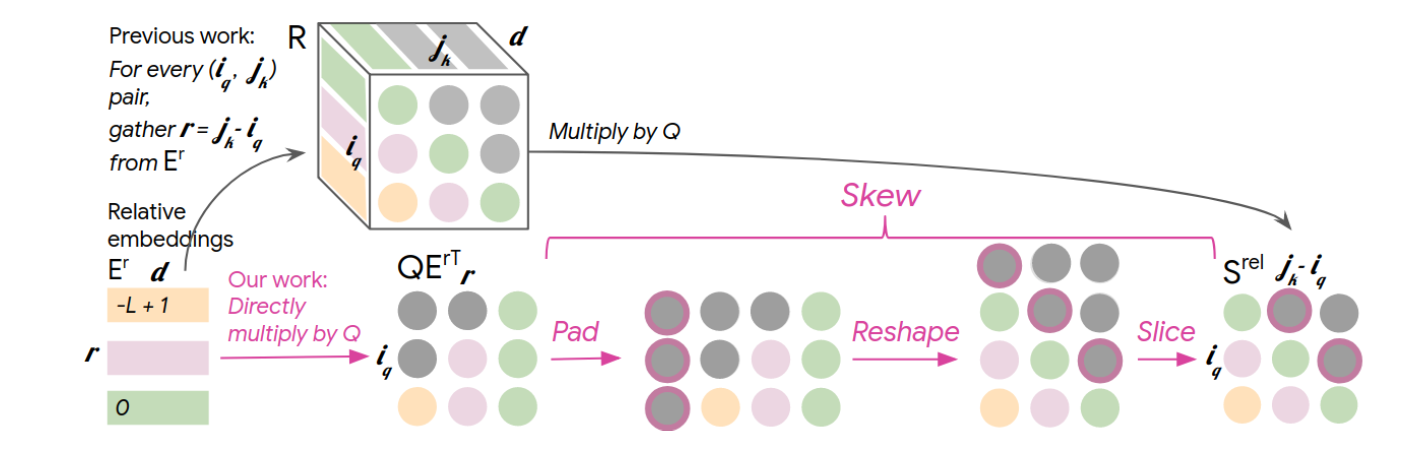
\includegraphics[width=0.9\textwidth]{imgs/skew_procedure.png}
    \caption{Skew Procedure from Huang et al.(2018) Gray indicates masked or padded positions, while each color corresponds to a different relative distance}
    \label{fig:fig4}
\end{figure}

\end{document}